\documentclass[../../main.tex]{subfiles}
\begin{document}
\section{Empirical and numerical examination of a Timoshenko beam} \label{sec:SP06}
Consider a study by Stephen and Puchegger in 2006, article \cite{SP06}. This study investigated the validity of the Timoshenko beam theory by hand of empirical and numerical data. The approach of the study is to compare the natural frequencies of a Timoshenko beam, to that of a three-dimensional elastic beam. The authors conducted comparisons between the models using theoretical methods as well as results from an empirical study on a physical beam, conducted by the authors.

The authors decided on a free-free beam configuration. The natural frequencies of the Timoshenko beam theory was obtained by using frequency equations from an article by Levison and Cooke \cite{LC81}. In theoretical approach of the three-dimensional beam, two methods were considered. A commercial finite elements method (ANSYS), and a resonant ultrasound spectroscopy (RUS) technique.

This section discusses the results of \cite{SP06}.

\subsection{Mathematical models}
Let $\Omega$ be the reference configuration of a free-free beam with square cross-section. The authors of \cite{SP06} do not formulate the models in the article. Consider Problem T-4 from section \ref{ssec:1D_Model:ModelProblems} for the free-free Timoshenko beam and Problem 3D-2 from section \ref{ssec:3D_Model:ModelProblems} for the free-free three-dimensional beam. The boundary conditions and reference configurations of the model problems are given below.

\subsubsection*{Problem T-4}
Find a function $u$, satisfying the equations of motion \eqref{eq:1D_Model:EquationOfMotion1D}- \eqref{eq:1D_Model:EquationOfMotion2D} and constitutive equations \eqref{eq:1D_Model:ConstitutiveEquations1D}- \eqref{eq:1D_Model:ConstitutiveEquations2D}.

{Free-Free Boundary Conditions:}
\begin{eqnarray}
	V(0,\cdot) = 0, \ \ &M(0,\cdot) = 0, \label{BC_1}\\
	V(1,\cdot) = 0, \ \ &M(1,\cdot) = 0. \label{BC_2}
\end{eqnarray}

\subsubsection{Problem 3D-2}
Find a vector valued function $u$, satisfying the equation of motion \eqref{eq:3D_Model:EM-D} and constitutive equation \eqref{eq:3D_Model:CE-D}. Let $\Omega$ represent the reference configuration of the beam with a square cross-section.
\begin{eqnarray*}
	\Omega := \left\{ \bar{x} = \langle x,y,z \rangle \in \mathbb{R} \ | \ 0 \leq x \leq 1, \ -\frac{h}{2} \leq y, z \leq \frac{h}{2}  \right\}
\end{eqnarray*}

with $h$ the height and width of the beam. $\partial \Omega$ denotes the boundary of $\Omega$. \\

{Free-Free Boundary Conditions:}\\
\begin{eqnarray*}
	Tn & = & 0 \quad \textrm{ on } \partial\Omega.
\end{eqnarray*} with $n$ a outward normal vector.


\subsection{Experimental setup}
Next the experiment conducted by \cite{SP06} is discussed. A short, aluminium alloy beam with near square cross-section is suspended at both ends. The beam is suspended by carbon fibre loops.

\begin{figure}[h!]
	\centering
	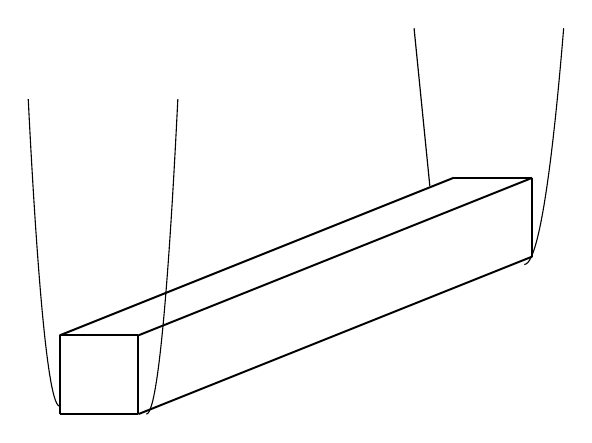
\begin{tikzpicture}
		
		\draw[line width = 0.25mm] (2,0) -- (7,2);
		\draw[line width = 0.25mm] (2,1) -- (7,3);
		\draw[line width = 0.25mm] (1,1) -- (6,3);
		
		\draw[line width = 0.25mm] (2,0) -- (2,1);
		\draw[line width = 0.25mm] (1,0) -- (1,1);
		\draw[line width = 0.25mm] (2,0) -- (1,0);
		\draw[line width = 0.25mm] (2,1) -- (1,1);
		
		\draw[line width = 0.25mm] (6,3) -- (7,3);
		\draw[line width = 0.25mm] (7,3) -- (7,2);
		
		\draw(2.1,0) parabola (2.5,4);
		\draw(1,0.1) parabola (0.6,4);
		
		\draw(6.9,1.9) parabola (7.4,4.9);
		\draw[line width = 0.15mm] (5.7,2.9) -- (5.5,4.9);
	
	\end{tikzpicture}
	\caption{Sketch of beam suspended at the end-points by carbon fibre loops.}
\end{figure} 
\FloatBarrier

To vibrate the beam, the authors of \cite{SP06} excited the carbon fibre loops and the frequencies were measured using two piezoelectric transducers. During the vibration, the beam will be momentarily free at both endpoints. The natural frequencies were obtained by sweeping through frequencies until a resonance was found.

The measured parameters of the beam is given in \cite{SP06}. Since the physical beam is only nearly square, the plane has two distinct planes. The plane of the beam with a larger diameter is referred to as the stiff plane and the plane of the beam with smaller diameter is referred to as the flexible plane, by \cite{SP06}.

For the flexible plane $\alpha = \pm 190$ and for the stiff plane $\alpha = \pm 189$. The parameter $\gamma = 0.2830$. The natural frequencies $f_k$ is defined as 
\begin{eqnarray*}
	f_k = \sqrt{\frac{\lambda_k}{2\pi}}
\end{eqnarray*} with $\lambda_k$ the $k$'th eigenvalue. These natural frequencies $f_k$ are dimensionless, and can be scaled back by multiplying the natural frequency $f_k$ by $t_0=\ell\sqrt{\frac{\rho}{G\kappa^2}}$, as defined in Chapter 1.

The cut-off frequency given in \cite{SP06} can be expressed as
\begin{eqnarray*}
	\omega_{co} = \sqrt{\frac{\kappa^2 A G}{\rho I}} = \frac{\alpha}{t_0}
\end{eqnarray*}
with the dimensionless cut-off frequency $\alpha$.

\subsection{Results from SP06}
The following table contains relevant results are obtained by \cite{SP06}. 
% Table generated by Excel2LaTeX from sheet 'Sheet1'
\begin{table}[htbp]
	\makebox[\textwidth]{
	\caption{Results from \cite{SP06} (excluding RUS).}
	\begin{tabular}{||c|c|cc|cc|c||}
		\hline
		{n} & {Measured} & {3D FEM} & {\% Error} & {Timoshenko Beam} & {\% Error} & Side \\
		\hline
		1     & 27359.6 & 27417.6 & 0,21\% & 27407.1 & 0,17\% & Flexible \\
		  	  & 27423.8 & 27515.6 & 0,33\% & 27505.3 & 0,30\% & Stiff \\
		2     & 60862   & 60882.0 & 0,03\% & 60851.1 & -0,02\% & Flexible \\
		 	  & 61098.3 & 61022.0 & -0,12\% & 60992.1 & -0,17\% & Stiff \\
		3     & 97609.5 & 97734.4 & 0,13\% & 97796.0 & 0,19\% & Flexible \\
			  & 97852.4 & 97881.5 & 0,03\% & 97945.4 & 0,09\% & Stiff \\
		4     & 161494 & 131658 & 0,12\% & 132277 & 0,60\% & Flexible \\
			  & 131732 & 131675 & -0,04\% & 132308 & 0,44\% & Stiff \\
		5     & 161352 & 161390 & 0,02\% & 163547 & 1,36\% & Stiff \\
			  & 161538 & 161517 & -0,01\% & 163611 & 1,31\% & Flexible \\
		6     & 165183 & 164887 & -0,18\% & 169108 & 2,38\% & Stiff \\
			  & 165598 & 165398 & -0,12\% & 169634 & 2,44\% & Flexible \\
		7     & 194863 & 194933 & 0,04\% & 202352 & 3,84\% & Flexible \\
		   	  & 194973 & 195032 & 0,03\% & 202115 & 3,66\% & Stiff \\
		8     & 195869 & 195977 & 0,06\% & 203319 & 3,80\% & Stiff \\
			  & 195908 & 196097 & 0,10\% & 203518 & 3,88\% & Flexible \\
		9     & 213501 &       &       & 241202 & 12,97\% & Flexible \\
			  & 213635 &       &       & 241067 & 12,84\% & Stiff \\
  {10 and 11} & 220556 &       &       & 247954 & 12,42\% & Flexible \\
			  & 220702 &       &       & 281542 & 27,57\% & Flexible \\
			  & 221010 &       &       & 247782 & 12,11\% & Stiff \\
			  & 221092 &       &       & 281408 & 27,28\% & Stiff \\
		\hline
	\end{tabular}%
	\label{tab:addlabel}%
}
\end{table}%

\FloatBarrier

Table 4.3 shows that the Timoshenko model compares well to the measured results from the experiment. The first 8 natural frequencies for the stiff and flexible planes are very close to the natural frequencies of the three-dimensional and physical beam.

\textcolor{red}{Onseker oor die***************}\\
In [LC81], a single frequency equation for the free-free beam is given. From the work in section \ref{sec:Timo:EigenvalueProblem}, it has been shown that there can be up to three-different frequency equations depending on $\alpha$. As the $\alpha$ for this beam is very small, the eigenvalues 9 and above will not be considered in this dissertation.\\
\textcolor{red}{Onseker oor die***************}
\end{document}

\begin{figure}[h!]
	\centering
	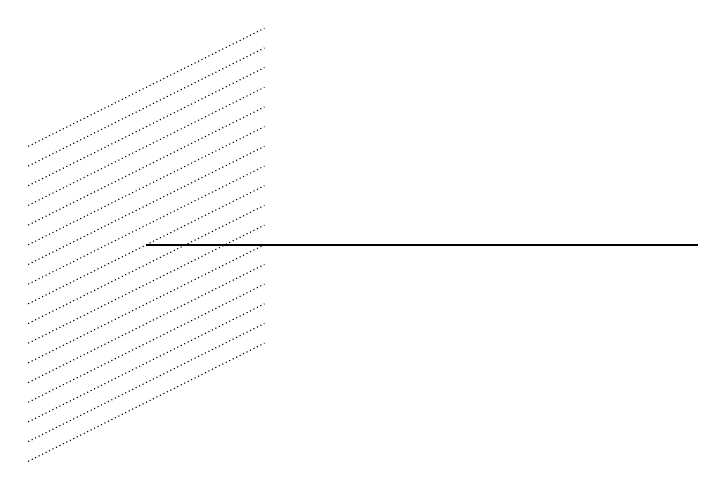
\begin{tikzpicture}
		
		\draw[line width = 0.3mm] (0,0) -- (7,0);
		
		
		\draw[scale=0.5, domain=-3:3, smooth, variable=\x,densely dotted] plot ({\x}, {0.5*\x+4});
		\draw[scale=0.5, domain=-3:3, smooth, variable=\x,densely dotted] plot ({\x}, {0.5*\x+3.5});
		\draw[scale=0.5, domain=-3:3, smooth, variable=\x,densely dotted] plot ({\x}, {0.5*\x+3});
		\draw[scale=0.5, domain=-3:3, smooth, variable=\x,densely dotted] plot ({\x}, {0.5*\x+2.5});
		\draw[scale=0.5, domain=-3:3, smooth, variable=\x,densely dotted] plot ({\x}, {0.5*\x+2});
		\draw[scale=0.5, domain=-3:3, smooth, variable=\x,densely dotted] plot ({\x}, {0.5*\x+1.5});
		\draw[scale=0.5, domain=-3:3, smooth, variable=\x,densely dotted] plot ({\x}, {0.5*\x+1});	
		\draw[scale=0.5, domain=-3:3, smooth, variable=\x,densely dotted] plot ({\x}, {0.5*\x+0.5});
		\draw[scale=0.5, domain=-3:3, smooth, variable=\x,densely dotted] plot ({\x}, {0.5*\x});
		\draw[scale=0.5, domain=-3:3, smooth, variable=\x,densely dotted] plot ({\x}, {0.5*\x-0.5});
		\draw[scale=0.5, domain=-3:3, smooth, variable=\x,densely dotted] plot ({\x}, {0.5*\x-1});
		\draw[scale=0.5, domain=-3:3, smooth, variable=\x,densely dotted] plot ({\x}, {0.5*\x-1.5});
		\draw[scale=0.5, domain=-3:3, smooth, variable=\x,densely dotted] plot ({\x}, {0.5*\x-2});
		\draw[scale=0.5, domain=-3:3, smooth, variable=\x,densely dotted] plot ({\x}, {0.5*\x-2.5});
		\draw[scale=0.5, domain=-3:3, smooth, variable=\x,densely dotted] plot ({\x}, {0.5*\x-3});
		\draw[scale=0.5, domain=-3:3, smooth, variable=\x,densely dotted] plot ({\x}, {0.5*\x-3.5});
		\draw[scale=0.5, domain=-3:3, smooth, variable=\x,densely dotted] plot ({\x}, {0.5*\x-4});
		
		
	\end{tikzpicture}
	\caption{Visual representation of beam suspended at the end-points by carbon fibre loops.}
\end{figure} 
\FloatBarrier

\begin{figure}[h!]
	\centering
	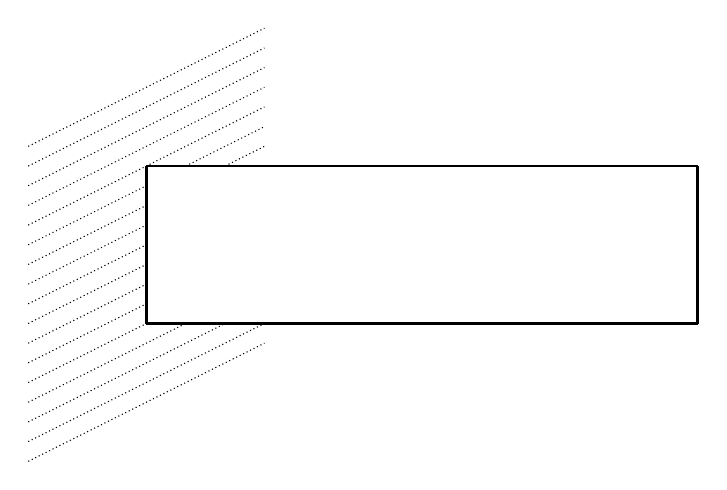
\begin{tikzpicture}
		
		\draw[line width = 0.3mm] (0,1) -- (7,1);
		\draw[line width = 0.3mm] (0,-1) -- (7,-1);
		\draw[line width = 0.3mm] (7,-1) -- (7,1);
		\draw[line width = 0.3mm] (0,-1) -- (0,1);
		
		
		\draw[scale=0.5, domain=-3:3, smooth, variable=\x,densely dotted] plot ({\x}, {0.5*\x+4});
		\draw[scale=0.5, domain=-3:3, smooth, variable=\x,densely dotted] plot ({\x}, {0.5*\x+3.5});
		\draw[scale=0.5, domain=-3:3, smooth, variable=\x,densely dotted] plot ({\x}, {0.5*\x+3});
		\draw[scale=0.5, domain=-3:3, smooth, variable=\x,densely dotted] plot ({\x}, {0.5*\x+2.5});
		\draw[scale=0.5, domain=-3:3, smooth, variable=\x,densely dotted] plot ({\x}, {0.5*\x+2});
		
		\draw[scale=0.5, domain=-3:0, smooth, variable=\x,densely dotted] plot ({\x}, {0.5*\x+1.5});
		\draw[scale=0.5, domain=-3:0, smooth, variable=\x,densely dotted] plot ({\x}, {0.5*\x+1});
		
		
		\draw[scale=0.5, domain=1:3, smooth, variable=\x,densely dotted] plot ({\x}, {0.5*\x+1.5});
		\draw[scale=0.5, domain=2:3, smooth, variable=\x,densely dotted] plot ({\x}, {0.5*\x+1});
		
		\draw[scale=0.5, domain=-3:0, smooth, variable=\x,densely dotted] plot ({\x}, {0.5*\x+0.5});
		\draw[scale=0.5, domain=-3:0, smooth, variable=\x,densely dotted] plot ({\x}, {0.5*\x});
		\draw[scale=0.5, domain=-3:0, smooth, variable=\x,densely dotted] plot ({\x}, {0.5*\x-0.5});
		\draw[scale=0.5, domain=-3:0, smooth, variable=\x,densely dotted] plot ({\x}, {0.5*\x-1});
		\draw[scale=0.5, domain=-3:0, smooth, variable=\x,densely dotted] plot ({\x}, {0.5*\x-1.5});
		\draw[scale=0.5, domain=-3:0, smooth, variable=\x,densely dotted] plot ({\x}, {0.5*\x-2});
		\draw[scale=0.5, domain=-3:1, smooth, variable=\x,densely dotted] plot ({\x}, {0.5*\x-2.5});
		\draw[scale=0.5, domain=-3:2, smooth, variable=\x,densely dotted] plot ({\x}, {0.5*\x-3});
		\draw[scale=0.5, domain=-3:3, smooth, variable=\x,densely dotted] plot ({\x}, {0.5*\x-3.5});
		\draw[scale=0.5, domain=-3:3, smooth, variable=\x,densely dotted] plot ({\x}, {0.5*\x-4});
		
		
		
	\end{tikzpicture}
	\caption{Visual representation of beam suspended at the end-points by carbon fibre loops.}
\end{figure} 
\FloatBarrier



\begin{figure}[h!]
	\centering
	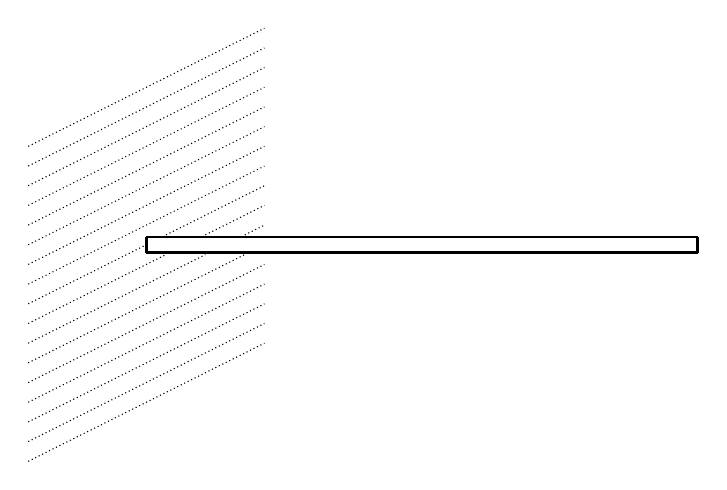
\begin{tikzpicture}
		
		\draw[line width = 0.3mm] (0,0.1) -- (7,0.1);
		\draw[line width = 0.3mm] (0,-0.1) -- (7,-0.1);
		\draw[line width = 0.3mm] (7,-0.1) -- (7,0.1);
		\draw[line width = 0.3mm] (0,-0.1) -- (0,0.1);
		
		
		\draw[scale=0.5, domain=-3:3, smooth, variable=\x,densely dotted] plot ({\x}, {0.5*\x+4});
		\draw[scale=0.5, domain=-3:3, smooth, variable=\x,densely dotted] plot ({\x}, {0.5*\x+3.5});
		\draw[scale=0.5, domain=-3:3, smooth, variable=\x,densely dotted] plot ({\x}, {0.5*\x+3});
		\draw[scale=0.5, domain=-3:3, smooth, variable=\x,densely dotted] plot ({\x}, {0.5*\x+2.5});
		\draw[scale=0.5, domain=-3:3, smooth, variable=\x,densely dotted] plot ({\x}, {0.5*\x+2});
		\draw[scale=0.5, domain=-3:3, smooth, variable=\x,densely dotted] plot ({\x}, {0.5*\x+1.5});
		\draw[scale=0.5, domain=-3:3, smooth, variable=\x,densely dotted] plot ({\x}, {0.5*\x+1});
		\draw[scale=0.5, domain=-3:3, smooth, variable=\x,densely dotted] plot ({\x}, {0.5*\x+0.5});
		
		\draw[scale=0.5, domain=-3:0, smooth, variable=\x,densely dotted] plot ({\x}, {0.5*\x});
		\draw[scale=0.5, domain=-3:0.5, smooth, variable=\x,densely dotted] plot ({\x}, {0.5*\x-0.5});
		\draw[scale=0.5, domain=-3:1.5, smooth, variable=\x,densely dotted] plot ({\x}, {0.5*\x-1});
		\draw[scale=0.5, domain=-3:2.5, smooth, variable=\x,densely dotted] plot ({\x}, {0.5*\x-1.5});
		
		\draw[scale=0.5, domain=0.5:3, smooth, variable=\x,densely dotted] plot ({\x}, {0.5*\x});
		\draw[scale=0.5, domain=1.5:3, smooth, variable=\x,densely dotted] plot ({\x}, {0.5*\x-0.5});
		\draw[scale=0.5, domain=2.5:3, smooth, variable=\x,densely dotted] plot ({\x}, {0.5*\x-1});
		
		
		\draw[scale=0.5, domain=-3:3, smooth, variable=\x,densely dotted] plot ({\x}, {0.5*\x-2});
		\draw[scale=0.5, domain=-3:3, smooth, variable=\x,densely dotted] plot ({\x}, {0.5*\x-2.5});
		\draw[scale=0.5, domain=-3:3, smooth, variable=\x,densely dotted] plot ({\x}, {0.5*\x-3});
		\draw[scale=0.5, domain=-3:3, smooth, variable=\x,densely dotted] plot ({\x}, {0.5*\x-3.5});
		\draw[scale=0.5, domain=-3:3, smooth, variable=\x,densely dotted] plot ({\x}, {0.5*\x-4});
		
		
		
	\end{tikzpicture}
	\caption{Visual representation of beam suspended at the end-points by carbon fibre loops.}
\end{figure} 
\FloatBarrier


\begin{figure}[h!]
	\centering
	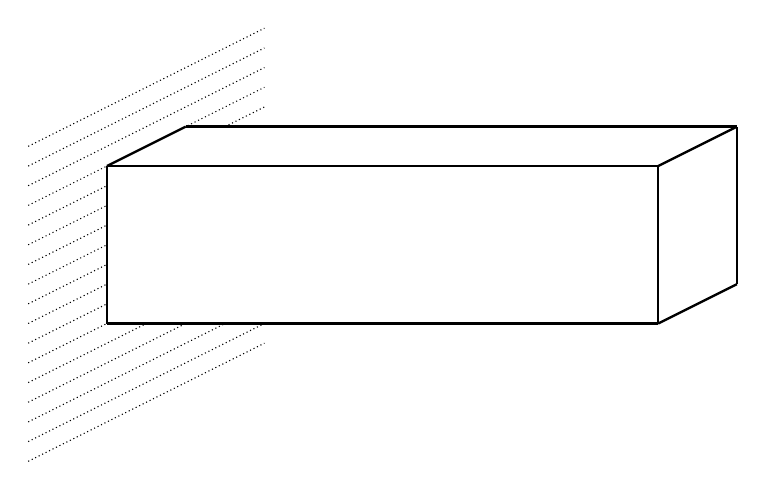
\begin{tikzpicture}
		
		\draw[line width = 0.3mm] (-0.5,1) -- (6.5,1);
		\draw[line width = 0.3mm] (-0.5,-1) -- (6.5,-1);
		\draw[line width = 0.3mm] (6.5,-1) -- (6.5,1);
		\draw[line width = 0.3mm] (-0.5,-1) -- (-0.5,1);
		
		\draw[line width = 0.3mm] (0.5,1.5) -- (7.5,1.5);
		\draw[line width = 0.3mm] (7.5,-0.5) -- (7.5,1.5);
		
		
		\draw[line width = 0.3mm] (-0.5,1) -- (0.5,1.5);
		\draw[line width = 0.3mm] (6.5,1) -- (7.5,1.5);
		\draw[line width = 0.3mm] (6.5,-1) -- (7.5,-0.5);
		
		
		
		\draw[scale=0.5, domain=-3:3, smooth, variable=\x,densely dotted] plot ({\x}, {0.5*\x+4});
		\draw[scale=0.5, domain=-3:3, smooth, variable=\x,densely dotted] plot ({\x}, {0.5*\x+3.5});
		\draw[scale=0.5, domain=-3:3, smooth, variable=\x,densely dotted] plot ({\x}, {0.5*\x+3});
		\draw[scale=0.5, domain=-3:3, smooth, variable=\x,densely dotted] plot ({\x}, {0.5*\x+2.5});
		
		\draw[scale=0.5, domain=-3:-1, smooth, variable=\x,densely dotted] plot ({\x}, {0.5*\x+2});
		\draw[scale=0.5, domain=2:3, smooth, variable=\x,densely dotted] plot ({\x}, {0.5*\x+2});
		
		\draw[scale=0.5, domain=-3:-1, smooth, variable=\x,densely dotted] plot ({\x}, {0.5*\x+1.5});
		\draw[scale=0.5, domain=-3:-1, smooth, variable=\x,densely dotted] plot ({\x}, {0.5*\x+1});
		\draw[scale=0.5, domain=-3:-1, smooth, variable=\x,densely dotted] plot ({\x}, {0.5*\x+0.5});
		\draw[scale=0.5, domain=-3:-1, smooth, variable=\x,densely dotted] plot ({\x}, {0.5*\x});
		\draw[scale=0.5, domain=-3:-1, smooth, variable=\x,densely dotted] plot ({\x}, {0.5*\x-0.5});
		\draw[scale=0.5, domain=-3:-1, smooth, variable=\x,densely dotted] plot ({\x}, {0.5*\x-1});
		\draw[scale=0.5, domain=-3:-1, smooth, variable=\x,densely dotted] plot ({\x}, {0.5*\x-1.5});
		\draw[scale=0.5, domain=-3:0, smooth, variable=\x,densely dotted] plot ({\x}, {0.5*\x-2});
		\draw[scale=0.5, domain=-3:1, smooth, variable=\x,densely dotted] plot ({\x}, {0.5*\x-2.5});
		\draw[scale=0.5, domain=-3:2, smooth, variable=\x,densely dotted] plot ({\x}, {0.5*\x-3});
		\draw[scale=0.5, domain=-3:3, smooth, variable=\x,densely dotted] plot ({\x}, {0.5*\x-3.5});
		\draw[scale=0.5, domain=-3:3, smooth, variable=\x,densely dotted] plot ({\x}, {0.5*\x-4});
		
		
		
	\end{tikzpicture}
	\caption{Visual representation of beam suspended at the end-points by carbon fibre loops.}
\end{figure} 
\FloatBarrier


\begin{figure}[h!]
	\centering
	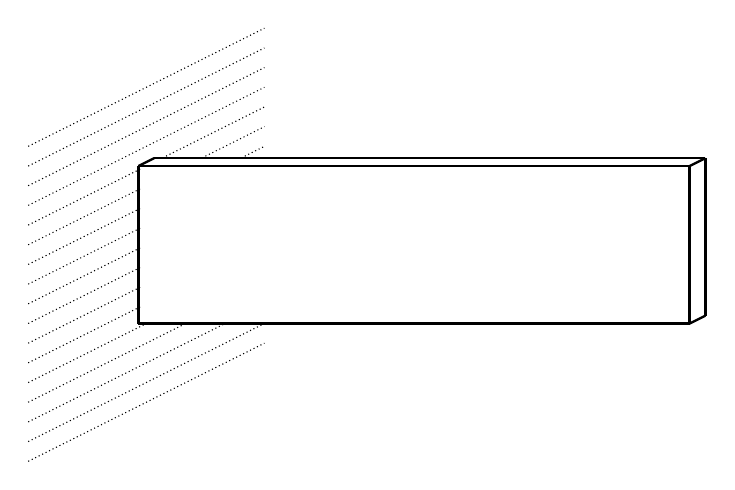
\begin{tikzpicture}
		
		\draw[line width = 0.3mm] (-0.1,1) -- (6.9,1);
		\draw[line width = 0.3mm] (-0.1,-1) -- (6.9,-1);
		\draw[line width = 0.3mm] (6.9,-1) -- (6.9,1);
		\draw[line width = 0.3mm] (-0.1,-1) -- (-0.1,1);
		
		\draw[line width = 0.3mm] (0.1,1.1) -- (7.1,1.1);
		\draw[line width = 0.3mm] (7.1,-0.9) -- (7.1,1.1);
		
		\draw[line width = 0.3mm] (-0.1,1) -- (0.1,1.1);
		\draw[line width = 0.3mm] (6.9,1) -- (7.1,1.1);
		\draw[line width = 0.3mm] (6.9,-1) -- (7.1,-0.9);
		
		
		
		\draw[scale=0.5, domain=-3:3, smooth, variable=\x,densely dotted] plot ({\x}, {0.5*\x+4});
		\draw[scale=0.5, domain=-3:3, smooth, variable=\x,densely dotted] plot ({\x}, {0.5*\x+3.5});
		\draw[scale=0.5, domain=-3:3, smooth, variable=\x,densely dotted] plot ({\x}, {0.5*\x+3});
		\draw[scale=0.5, domain=-3:3, smooth, variable=\x,densely dotted] plot ({\x}, {0.5*\x+2.5});
		
		\draw[scale=0.5, domain=-3:-0.1, smooth, variable=\x,densely dotted] plot ({\x}, {0.5*\x+2});
		\draw[scale=0.5, domain=-3:-0.1, smooth, variable=\x,densely dotted] plot ({\x}, {0.5*\x+1.5});
		\draw[scale=0.5, domain=-3:-0.1, smooth, variable=\x,densely dotted] plot ({\x}, {0.5*\x+1});
		
		\draw[scale=0.5, domain=0.5:3, smooth, variable=\x,densely dotted] plot ({\x}, {0.5*\x+2});
		\draw[scale=0.5, domain=1.5:3, smooth, variable=\x,densely dotted] plot ({\x}, {0.5*\x+1.5});
		\draw[scale=0.5, domain=2.5:3, smooth, variable=\x,densely dotted] plot ({\x}, {0.5*\x+1});
		
		\draw[scale=0.5, domain=-3:-0.1, smooth, variable=\x,densely dotted] plot ({\x}, {0.5*\x+0.5});
		\draw[scale=0.5, domain=-3:-0.1, smooth, variable=\x,densely dotted] plot ({\x}, {0.5*\x});
		\draw[scale=0.5, domain=-3:-0.1, smooth, variable=\x,densely dotted] plot ({\x}, {0.5*\x-0.5});
		\draw[scale=0.5, domain=-3:-0.1, smooth, variable=\x,densely dotted] plot ({\x}, {0.5*\x-1});
		\draw[scale=0.5, domain=-3:-0.1, smooth, variable=\x,densely dotted] plot ({\x}, {0.5*\x-1.5});
		\draw[scale=0.5, domain=-3:0, smooth, variable=\x,densely dotted] plot ({\x}, {0.5*\x-2});
		\draw[scale=0.5, domain=-3:1, smooth, variable=\x,densely dotted] plot ({\x}, {0.5*\x-2.5});
		\draw[scale=0.5, domain=-3:2, smooth, variable=\x,densely dotted] plot ({\x}, {0.5*\x-3});
		\draw[scale=0.5, domain=-3:3, smooth, variable=\x,densely dotted] plot ({\x}, {0.5*\x-3.5});
		\draw[scale=0.5, domain=-3:3, smooth, variable=\x,densely dotted] plot ({\x}, {0.5*\x-4});
		
		
		
	\end{tikzpicture}
	\caption{Visual representation of beam suspended at the end-points by carbon fibre loops.}
\end{figure} 
\FloatBarrier


\begin{figure}[h!]
	\centering
	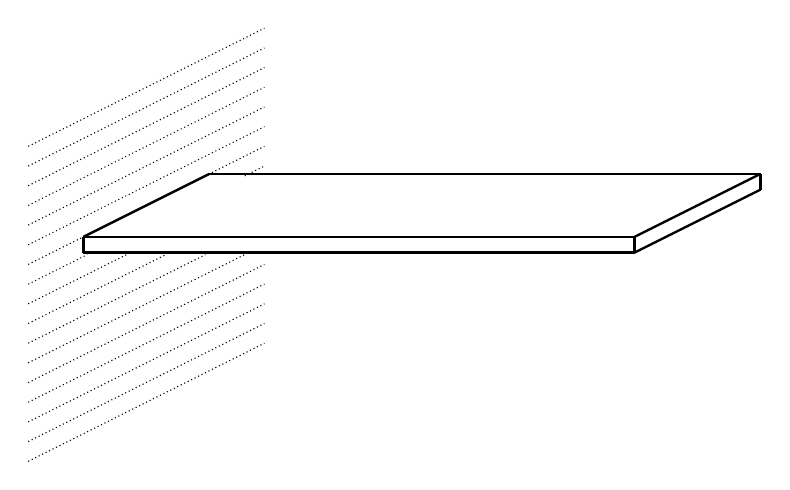
\begin{tikzpicture}
		
		\draw[line width = 0.3mm] (-0.8,0.1) -- (6.2,0.1);
		\draw[line width = 0.3mm] (-0.8,-0.1) -- (6.2,-0.1);
		\draw[line width = 0.3mm] (6.2,-0.1) -- (6.2,0.1);
		\draw[line width = 0.3mm] (-0.8,-0.1) -- (-0.8,0.1);
		
		\draw[line width = 0.3mm] (0.8,0.9) -- (7.8,0.9);
		\draw[line width = 0.3mm] (7.8,0.7) -- (7.8,0.9);
		
		\draw[line width = 0.3mm] (-0.8,0.1) -- (0.8,0.9);
		\draw[line width = 0.3mm] (6.2,0.1) -- (7.8,0.9);
		\draw[line width = 0.3mm] (6.2,-0.1) -- (7.8,0.7);
		
		
		
		\draw[scale=0.5, domain=-3:3, smooth, variable=\x,densely dotted] plot ({\x}, {0.5*\x+4});
		\draw[scale=0.5, domain=-3:3, smooth, variable=\x,densely dotted] plot ({\x}, {0.5*\x+3.5});
		\draw[scale=0.5, domain=-3:3, smooth, variable=\x,densely dotted] plot ({\x}, {0.5*\x+3});
		\draw[scale=0.5, domain=-3:3, smooth, variable=\x,densely dotted] plot ({\x}, {0.5*\x+2.5});
		\draw[scale=0.5, domain=-3:3, smooth, variable=\x,densely dotted] plot ({\x}, {0.5*\x+2});
		\draw[scale=0.5, domain=-3:3, smooth, variable=\x,densely dotted] plot ({\x}, {0.5*\x+1.5});
		\draw[scale=0.5, domain=-3:3, smooth, variable=\x,densely dotted] plot ({\x}, {0.5*\x+1});
		
		\draw[scale=0.5, domain=-3:-1.5, smooth, variable=\x,densely dotted] plot ({\x}, {0.5*\x+0.5});
		\draw[scale=0.5, domain=2.5:3, smooth, variable=\x,densely dotted] plot ({\x}, {0.5*\x+0.5});
		
		\draw[scale=0.5, domain=-3:-0.5, smooth, variable=\x,densely dotted] plot ({\x}, {0.5*\x});
		\draw[scale=0.5, domain=-3:0.5, smooth, variable=\x,densely dotted] plot ({\x}, {0.5*\x-0.5});
		\draw[scale=0.5, domain=-3:1.5, smooth, variable=\x,densely dotted] plot ({\x}, {0.5*\x-1});
		\draw[scale=0.5, domain=-3:2.5, smooth, variable=\x,densely dotted] plot ({\x}, {0.5*\x-1.5});
		\draw[scale=0.5, domain=-3:3, smooth, variable=\x,densely dotted] plot ({\x}, {0.5*\x-2});
		\draw[scale=0.5, domain=-3:3, smooth, variable=\x,densely dotted] plot ({\x}, {0.5*\x-2.5});
		\draw[scale=0.5, domain=-3:3, smooth, variable=\x,densely dotted] plot ({\x}, {0.5*\x-3});
		\draw[scale=0.5, domain=-3:3, smooth, variable=\x,densely dotted] plot ({\x}, {0.5*\x-3.5});
		\draw[scale=0.5, domain=-3:3, smooth, variable=\x,densely dotted] plot ({\x}, {0.5*\x-4});
		
	\end{tikzpicture}
	\caption{Visual representation of beam suspended at the end-points by carbon fibre loops.}
\end{figure} 
\FloatBarrier

\begin{figure}[h!]
	\centering
	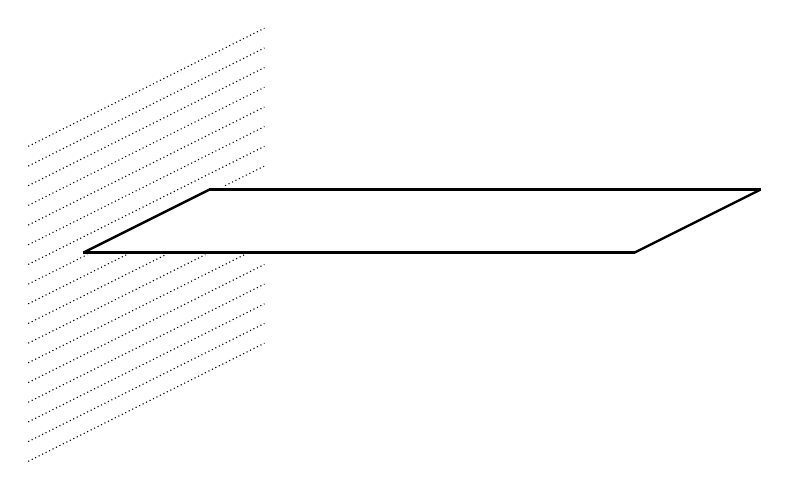
\begin{tikzpicture}
		
		\draw[line width = 0.3mm] (-0.8,-0.1) -- (6.2,-0.1);
		\draw[line width = 0.3mm] (0.8,0.7) -- (7.8,0.7);
		\draw[line width = 0.3mm] (-0.8,-0.1) -- (0.8,0.7);
		\draw[line width = 0.3mm] (6.2,-0.1) -- (7.8,0.7);
		
		
		
		\draw[scale=0.5, domain=-3:3, smooth, variable=\x,densely dotted] plot ({\x}, {0.5*\x+4});
		\draw[scale=0.5, domain=-3:3, smooth, variable=\x,densely dotted] plot ({\x}, {0.5*\x+3.5});
		\draw[scale=0.5, domain=-3:3, smooth, variable=\x,densely dotted] plot ({\x}, {0.5*\x+3});
		\draw[scale=0.5, domain=-3:3, smooth, variable=\x,densely dotted] plot ({\x}, {0.5*\x+2.5});
		\draw[scale=0.5, domain=-3:3, smooth, variable=\x,densely dotted] plot ({\x}, {0.5*\x+2});
		\draw[scale=0.5, domain=-3:3, smooth, variable=\x,densely dotted] plot ({\x}, {0.5*\x+1.5});
		\draw[scale=0.5, domain=-3:3, smooth, variable=\x,densely dotted] plot ({\x}, {0.5*\x+1});
		
		\draw[scale=0.5, domain=-3:-1.5, smooth, variable=\x,densely dotted] plot ({\x}, {0.5*\x+0.5});
		\draw[scale=0.5, domain=2:3, smooth, variable=\x,densely dotted] plot ({\x}, {0.5*\x+0.5});
		
		\draw[scale=0.5, domain=-3:-0.5, smooth, variable=\x,densely dotted] plot ({\x}, {0.5*\x});
		\draw[scale=0.5, domain=-3:0.5, smooth, variable=\x,densely dotted] plot ({\x}, {0.5*\x-0.5});
		\draw[scale=0.5, domain=-3:1.5, smooth, variable=\x,densely dotted] plot ({\x}, {0.5*\x-1});
		\draw[scale=0.5, domain=-3:2.5, smooth, variable=\x,densely dotted] plot ({\x}, {0.5*\x-1.5});
		\draw[scale=0.5, domain=-3:3, smooth, variable=\x,densely dotted] plot ({\x}, {0.5*\x-2});
		\draw[scale=0.5, domain=-3:3, smooth, variable=\x,densely dotted] plot ({\x}, {0.5*\x-2.5});
		\draw[scale=0.5, domain=-3:3, smooth, variable=\x,densely dotted] plot ({\x}, {0.5*\x-3});
		\draw[scale=0.5, domain=-3:3, smooth, variable=\x,densely dotted] plot ({\x}, {0.5*\x-3.5});
		\draw[scale=0.5, domain=-3:3, smooth, variable=\x,densely dotted] plot ({\x}, {0.5*\x-4});
		
	\end{tikzpicture}
	\caption{Visual representation of beam suspended at the end-points by carbon fibre loops.}
\end{figure} 
\FloatBarrier
